\documentclass[sigconf,nonacm]{webmedia}

\usepackage{amsmath}
\usepackage{xurl}
\usepackage{pgfplots}
\pgfplotsset{compat=1.18}
\graphicspath{{../graficos/}{../}}

%webmedia.cls is adapted from acmart.cls for use in Proceedings of the Brazilian Symposium on Multimedia and the Web (WebMedia)

%%
%% \BibTeX command to typeset the BibTeX logo in the docs
\AtBeginDocument{%
  \providecommand\BibTeX{{%
    \normalfont B\kern-0.5em{\scshape i\kern-0.25em b}\kern-0.8em\TeX}}}

\settopmatter{printacmref=false, printfolios=false}

%% Choose the appropriate event.
%\setevent{webmedia}
%\proceedingsDetails[WebMedia’2026]{Proceedings of the Brazilian Symposium on Multimedia and the Web}{2026}{Lavras/MG, Brazil} 
%\ISSN{2966-2753}

\begin{document}

%%
%% The "title" command has an optional parameter,
%% allowing the author to define a "short title" to be used in page headers.
\title{Relatório de Análise Estrutural e Algorítmica: A Rede Zachary's Karate Club}

%%
%% The "author" command and its associated commands are used to define
%% the authors and their affiliations.
\author{Magno Macedo Miranda}
\email{magno.miranda@ufba.br}
\affiliation{%
  \institution{Universidade Federal da Bahia (UFBA)}
  \city{Salvador}
  \state{Bahia}
  \country{Brasil}
}

\renewcommand{\shortauthors}{Macedo}

%%
%% The abstract is a short summary of the work to be presented in the
%% article.
\begin{abstract}
  Este relatório apresenta uma análise da rede social {Zachary's Karate Club} usando a biblioteca Python {Karate Club}. O documento está dividido em três partes. Na Parte I, foi feita a caracterização da estrutura do grafo, calculando e analisando métricas fundamentais como densidade, diâmetro, comprimento médio dos caminhos, agrupamento local e distribuição de conexões. Na Parte II, foi detalhada a implementação manual de oito algoritmos clássicos de grafos (BFS, DFS, Eulerianidade, Dijkstra, Bellman-Ford, Floyd-Warshall, Tarjan SCC e Kruskal MST), comparando seus tempos teóricos e práticos em 50 rodadas de testes. Na Parte III, foi realizada uma análise de propriedades da rede como pequeno mundo ({small-world}), lei de potência, robustez contra falhas e ataques direcionados, e comparação com os modelos clássicos de redes (Erdős-Rényi, Watts-Strogatz e Barabási-Albert), relacionando os dados com a divisão histórica real do clube.
\end{abstract}

%%
%% Keywords. The author(s) should pick words that accurately describe
%% the work being presented. Separate the keywords with commas.
\keywords{Teoria dos Grafos, Zachary's Karate Club, Algoritmos de Grafos, Benchmark de Desempenho, Análise Estatística}

%%
%% This command processes the author and affiliation and title
%% information and builds the first part of the formatted document.
\maketitle

\section{Introdução}

A modelagem de sistemas complexos por meio de grafos permite caracterizar de forma quantitativa as relações entre entidades em redes sociais, biológicas e de transporte. O artigo \cite{Rozemberczki2020} apresenta um arcabouço focado em algoritmos de aprendizado não supervisionado sobre grafos, tais como detecção de comunidades e incorporação de nós. 

O nome da biblioteca é diretamente inspirado na rede  {Zachary's Karate Club} \cite{Zachary1977}, um grafo que mapeia as amizades entre 34 membros de um clube universitário durante a década de 1970. Devido a uma disputa entre o instrutor ("Mr. Hi") e o administrador ("John A."), o clube dividiu-se em duas "facções". Esta rede tornou-se o principal  {benchmark} para validar algoritmos de agrupamento em grafos.

Este relatório divide-se nas três partes requeridas para a avaliação: a caracterização estrutural básica (Parte I), o benchmark experimental dos algoritmos da disciplina (Parte II) e a modelagem estrutural avançada (Parte III).

\medskip
\noindent\textbf{Repositório:} todos os códigos-fonte, scripts, conjunto de dados tratados e este relatório estão disponíveis publicamente em: \url{https://github.com/maccedoz/Analisando-Grafos-do-SNAP-MATA53}

\section{Metodologia e Tratamento de Dados}

O grafo original do clube de caratê de Zachary foi obtido diretamente da biblioteca NetworkX (\path{nx.karate_club_graph()}), onde a rede é modelada como um grafo não-ponderado, não-direcionado e simples, composto por 34 nós (rotulados de 0 a 33) e 78 arestas.

\subsection{Tabela de Tratamentos Realizados}

A Tabela \ref{tab:tratamentos} detalha cada etapa de tratamento considerada, seu status de aplicação e a respectiva justificativa técnica.

\begin{table*}[t]
  \caption{Checklist de Tratamento de Dados do Grafo Zachary's Karate Club}
  \label{tab:tratamentos}
  \begin{tabular}{llp{8cm}}
    \toprule
    Tratamento Considerado & Status & Justificativa \\
    \midrule
    Grafo temporal $\rightarrow$ estático & Não Aplicável & O Zachary's Karate Club é uma rede estática, trata-se de um único  {snapshot} das relações sociais coletadas entre 1970--1972. Não há dimensão temporal nos dados. \\
    Grafo dirigido $\rightarrow$ não-direcionado & Não Aplicável & O grafo já é originalmente não-direcionado. As amizades no clube são relações simétricas (mútuas), confirmado por \path{G.is_directed() = False}. \\
    Multigrafo $\rightarrow$ grafo simples & Não Aplicável & O grafo já é simples por construção. Não existem arestas paralelas entre nenhum par de nós, confirmado por \path{G.is_multigraph() = False}. \\
    Remoção de auto-loops & Não Aplicável & Não há auto-loops (arestas de um nó para si mesmo) no dataset. Verificado: \path{nx.number_of_selfloops(G) = 0}. \\
    Extração da maior componente conexa & Não Aplicável & O grafo original é totalmente conexo, possuindo exatamente 1 componente conexo de tamanho 34, abrangendo todos os nós. Nenhuma extração foi necessária. \\
    Filtragem por intervalo temporal & Não Aplicável & Não há marcações temporais nas arestas ou nós. O dataset representa um período fixo de observação (1970--1972) sem granularidade temporal. \\
    Geração de pesos nas arestas & \textbf{Realizado} & Como a rede original é não-ponderada, foram atribuídos pesos determinísticos via $w(u, v) = (u + v) \bmod 5 + 1$, gerando valores inteiros em $[1, 5]$. Isso permite rodar os algoritmos de caminho mínimo (Dijkstra, Bellman-Ford, Floyd-Warshall) e a MST (Kruskal). \\
    Mapeamento de atributos sociais & \textbf{Realizado} & Foi extraído o atributo \path{club} de cada nó do NetworkX, mapeando o grupo final de cada membro ( {"Mr. Hi"} ou  {"Officer"}) para usar nas visualizações e na análise da divisão social. \\
    Conversão para lista de adjacência & \textbf{Realizado} & A representação em lista de adjacência foi exportada para \path{data/karate_adj_list.txt}, onde cada linha registra um nó e seus vizinhos. Este formato é usado como entrada direta dos algoritmos implementados do zero. \\
    Exportação para formato estruturado (CSV) & \textbf{Realizado} & A rede tratada foi exportada para \path{data/karate_club_edges.csv} com as colunas \path{source}, \path{target}, \path{weight}, \path{source_club} e \path{target_club}, servindo como base de dados persistida do projeto. \\
    \bottomrule
  \end{tabular}
\end{table*}

\subsection{Detalhamento dos Tratamentos Realizados}

Dentre os tratamentos listados, quatro foram efetivamente executados sobre o dataset por meio do script \path{scripts/gerar_dataset.py}:

Primeiramente, foi feita a \textbf{geração de pesos nas arestas}: como a rede original é não-ponderada, a força da relação foi simulada colocando pesos determinísticos positivos em cada aresta $(u, v)$ usando a expressão:
\begin{equation}
    w(u, v) = (u + v) \bmod 5 + 1
\end{equation}
Esta fórmula gera valores inteiros de $1$ a $5$, o que permite testar algoritmos de menor caminho (Dijkstra, Bellman-Ford, Floyd-Warshall) e árvore geradora mínima (Kruskal). Também foi feito o \textbf{mapeamento de atributos sociais}: o atributo \path{club} de cada nó foi extraído, indicando a facção final de cada membro após a divisão histórica do clube. A rede também foi convertida para \textbf{lista de adjacência} no arquivo \path{data/karate_adj_list.txt}. Cada linha do arquivo segue o formato {nó: [vizinhos]}, mostrando as conexões de cada vértice e servindo de entrada direta para os algoritmos. Por fim, a rede foi salva em \textbf{CSV estruturado} no arquivo \path{data/karate_club_edges.csv}, contendo as colunas \path{source}, \path{target}, \path{weight}, \path{source_club} e \path{target_club}, garantindo uma base de dados pronta para reuso.

\section{Parte I - Análise Estrutural Obrigatória}
\label{sec:parte_i}

Nesta primeira etapa, foram calculadas as principais métricas da estrutura da rede de Zachary. As métricas incluem o \textbf{Número de Vértices ($N$)}, que indica o total de nós ($N = |V|$), e o \textbf{Número de Arestas ($M$)}, que indica o total de conexões ($M = |E|$). A partir deles, define-se o \textbf{Grau Médio ($\langle k \rangle$)} como a média de conexões de todos os nós, dada por $\langle k \rangle = \frac{2M}{N}$, e a \textbf{Densidade ($D$)} como a razão entre as conexões existentes e o total máximo de conexões possíveis:
\begin{equation}
    D = \frac{2M}{N(N - 1)}
\end{equation}
A conectividade é avaliada pelos \textbf{Componentes Conexos}, que indicam as partes da rede que estão interligadas. Usando a menor distância $d(u,v)$ entre os nós, define-se o \textbf{Diâmetro ($d$)} como a maior distância entre qualquer par de nós, dada por:
\begin{equation}
    d = \max_{u, v \in V} d(u, v)
\end{equation}
e o \textbf{Raio ($r$)} como a menor das maiores distâncias de um nó para os demais:
\begin{equation}
    r = \min_{u \in V} \max_{v \in V} d(u, v)
\end{equation}
O \textbf{Comprimento Médio dos Caminhos ($L$)} representa a distância média calculada para todos os pares de nós na rede:
\begin{equation}
    L = \frac{1}{N(N - 1)} \sum_{u \neq v} d(u, v)
\end{equation}
A proximidade dos nós é medida pelo \textbf{Coeficiente de Clusterização Médio ($\langle C \rangle$)}, que é a média dos coeficientes de agrupamento de cada nó $C_i$:
\begin{equation}
    C_i = \frac{2 T_i}{k_i (k_i - 1)}
\end{equation}
onde $T_i$ é o número de triângulos passando pelo nó $i$. Por fim, o \textbf{Número de Triângulos ($T$)} conta o total de grupos de três nós totalmente conectados entre si.

A Tabela \ref{tab:metrics} resume os resultados obtidos. O grafo é totalmente conectado (único componente com todos os 34 nós) e tem densidade de $13,9\%$. O baixo diâmetro ($d = 5$) e a distância média curta ($L \approx 2,41$) mostram que a rede é de "mundo pequeno". Além disso, o alto coeficiente de clusterização ($\langle C \rangle \approx 0,571$) mostra que há uma forte tendência de formação de pequenos grupos de amigos. O número total de triângulos na rede é 45.

\begin{figure}[h]
  \centering
  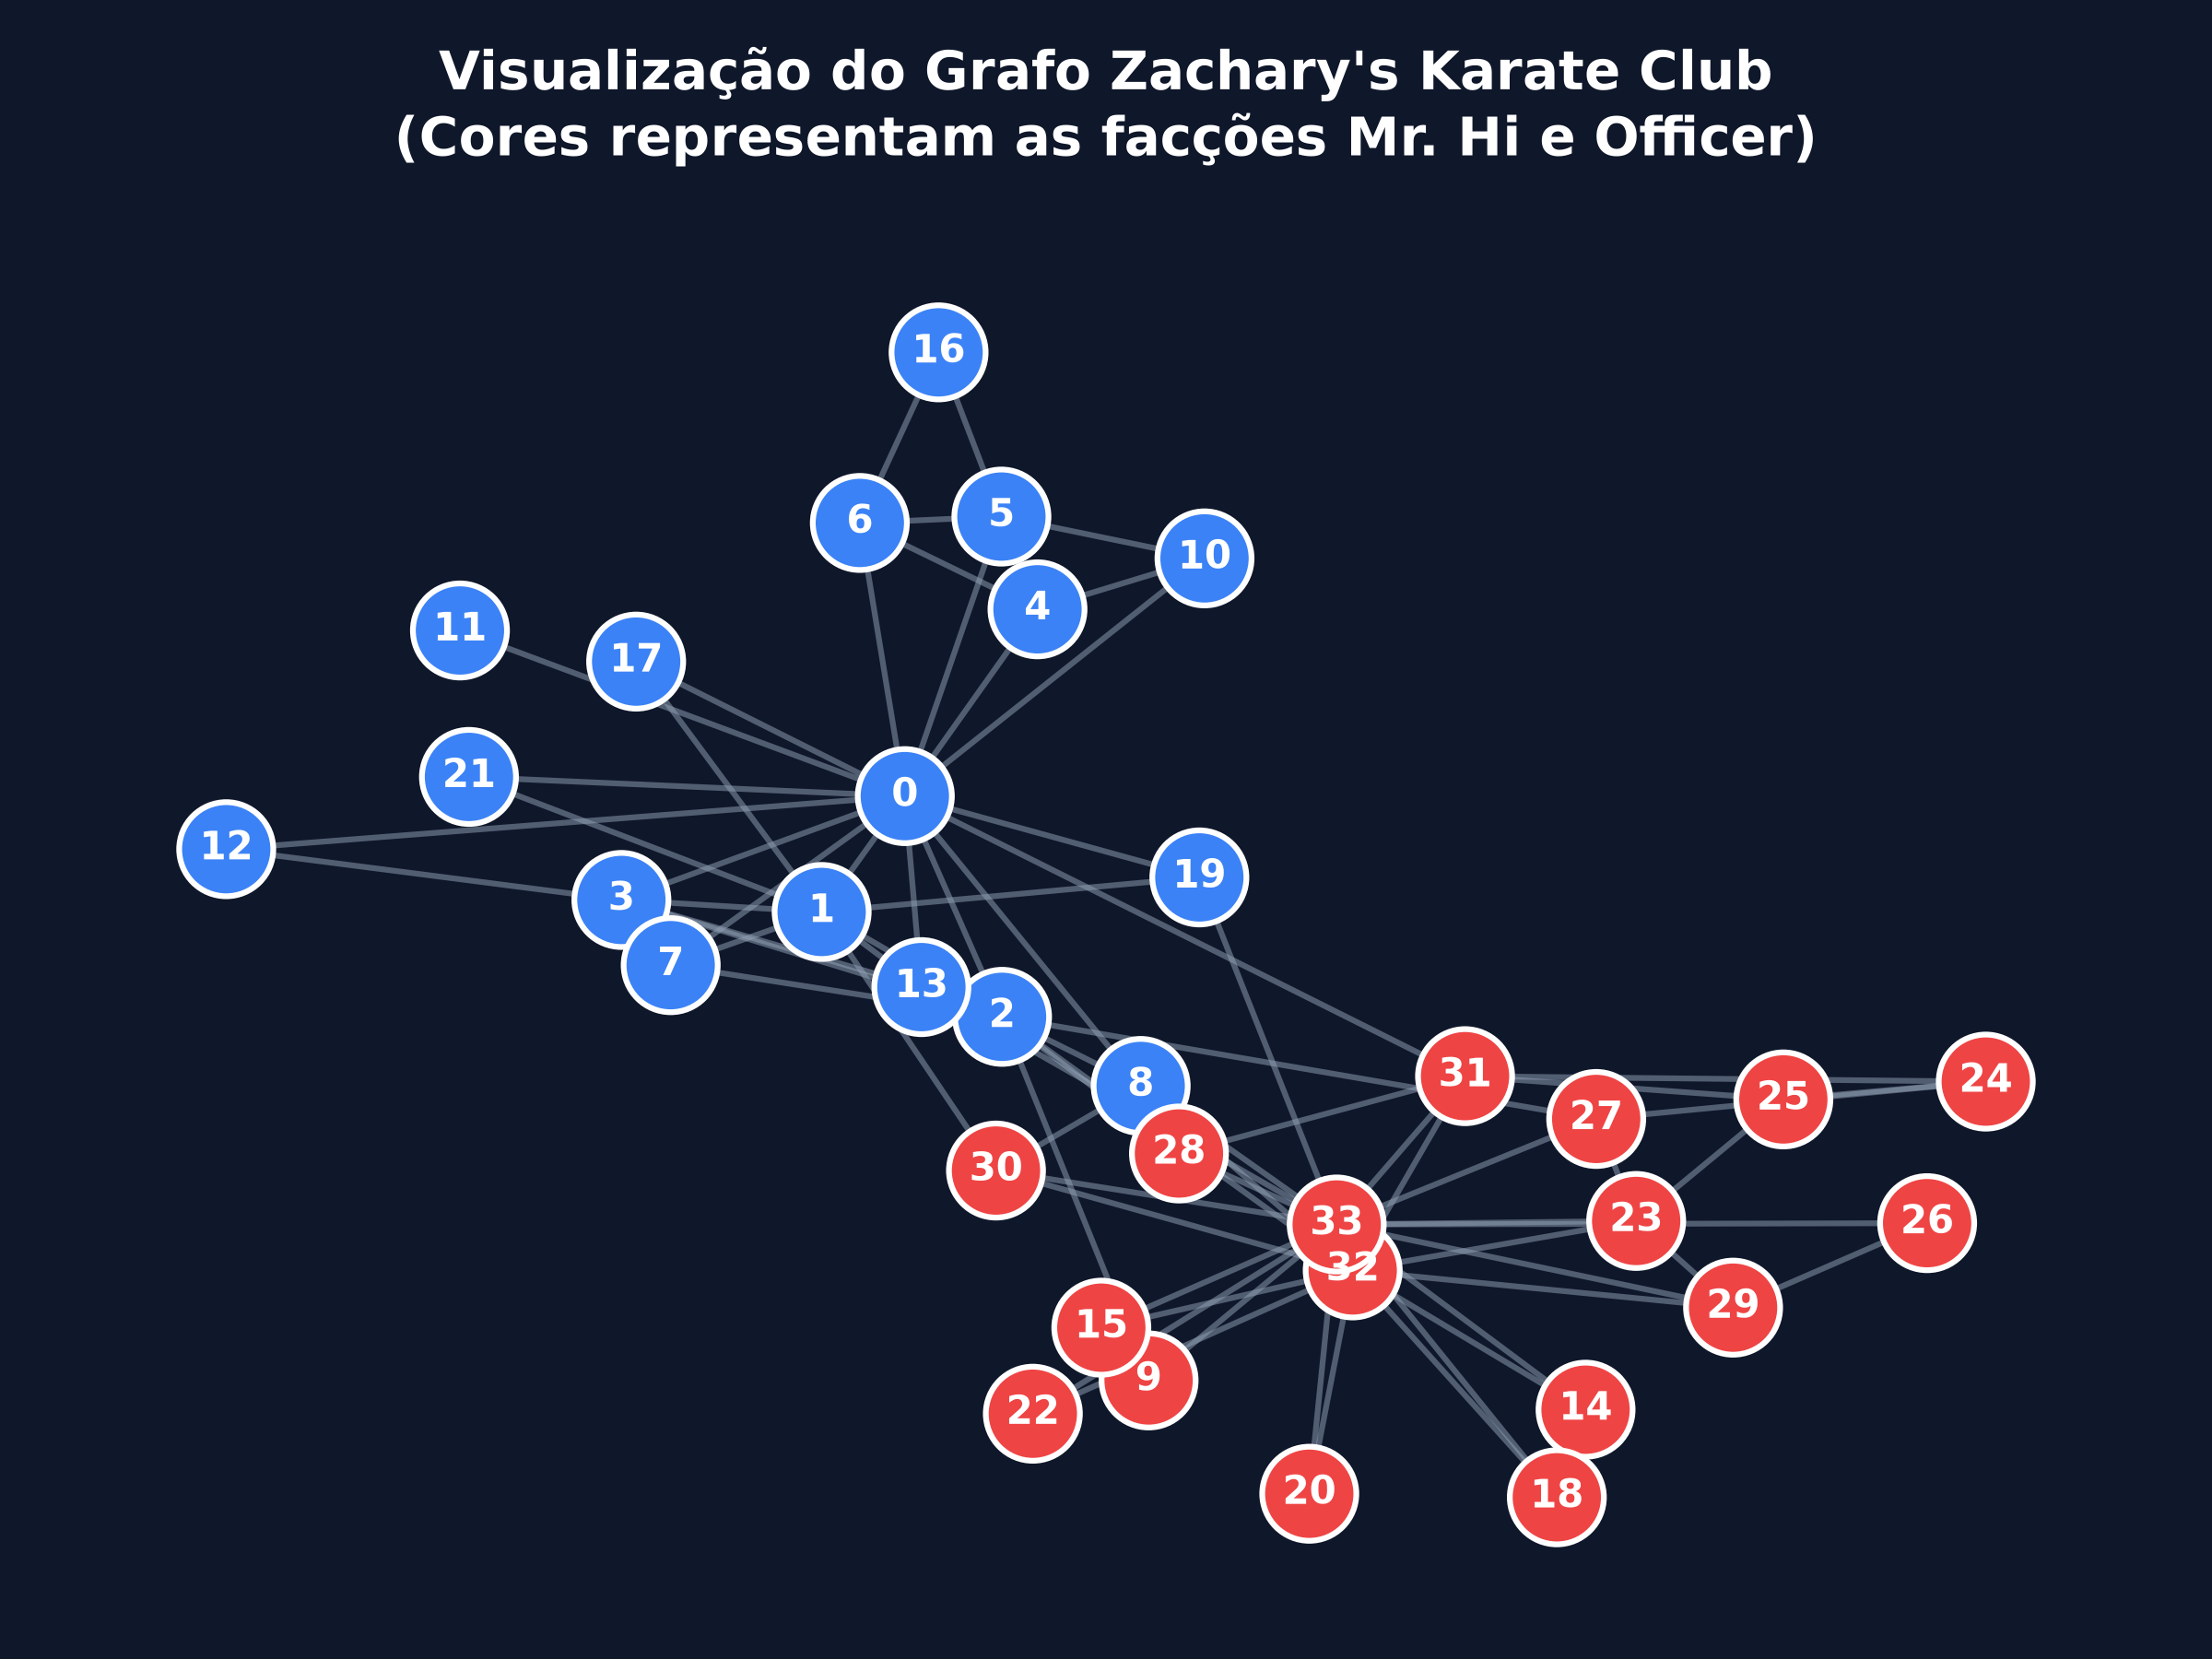
\includegraphics[width=0.9\linewidth]{karate_club_graph}
  \caption{Estrutura do Grafo Zachary's Karate Club. Cores representam as facções Mr. Hi (Azul) e John A. (Vermelho).}
  \label{fig:karate_graph}
\end{figure}

A estrutura mostrada na Figura \ref{fig:karate_graph} (gerada com o script \path{scripts/gerar_graficos.py}) deixa clara a divisão social que levou à separação do grupo de caratê.

\begin{table*}[t]
  \caption{Métricas Estruturais Computadas para o Grafo Zachary's Karate Club}
  \label{tab:metrics}
  \begin{tabular}{llcl}
    \toprule
    Métrica Solicitada & Status & Valor Computado & Justificativa / Comentário \\
    \midrule
    Número de Vértices & Computado & 34 & Obtido diretamente de $|V|$. \\
    Número de Arestas & Computado & 78 & Obtido diretamente de $|E|$. \\
    Grau Mínimo & Computado & 1 & Menor número de conexões observadas em um único nó. \\
    Grau Máximo & Computado & 17 & Maior número de conexões (nó hub central). \\
    Grau Médio & Computado & 4,588 & Média aritmética dos graus de todos os nós ($\langle k \rangle$). \\
    Distribuição de Grafos/Graus & Computado & Ver Seção \ref{sec:degree_dist} & Distribuição empírica da frequência de graus. \\
    Densidade & Computado & 0,139 & Relação de arestas existentes sobre possíveis ($D$). \\
    Número de Componentes Conexos & Computado & 1 & A rede é totalmente conexa. \\
    Tamanho de Cada Componente & Computado & [34] & O componente conexo único contém todos os nós. \\
    Diâmetro & Computado & 5 & Maior distância geodésica entre dois nós ($d$). \\
    Raio & Computado & 3 & Excentricidade mínima entre todos os nós ($r$). \\
    Comprimento Médio dos Caminhos & Computado & 2,408 & Distância média entre todos os pares de nós ($L$). \\
    Coeficiente de Clusterização Médio & Computado & 0,571 & Média local de agrupamento ($\langle C \rangle$). \\
    Número de Triângulos & Computado & 45 & Número total de cliques de tamanho 3 ($T$). \\
    \bottomrule
  \end{tabular}
\end{table*}

\subsection{Distribuição de Graus}
\label{sec:degree_dist}

A distribuição de graus está detalhada na Tabela \ref{tab:degree_freq} e ilustrada graficamente na Figura \ref{fig:degree_dist}.

\begin{table}[h]
  \caption{Frequência de Nós por Grau}
  \label{tab:degree_freq}
  \begin{tabular}{ccc}
    \toprule
    Grau ($k$) & Frequência (Nós) & Proporção (\%) \\
    \midrule
    1 & 1 & 2,94\% \\
    2 & 11 & 32,35\% \\
    3 & 6 & 17,65\% \\
    4 & 6 & 17,65\% \\
    5 & 3 & 8,82\% \\
    6 & 2 & 5,88\% \\
    9 & 1 & 2,94\% \\
    10 & 1 & 2,94\% \\
    12 & 1 & 2,94\% \\
    16 & 1 & 2,94\% \\
    17 & 1 & 2,94\% \\
    \bottomrule
  \end{tabular}
\end{table}

A distribuição, cujo comportamento empírico é ilustrado na Figura \ref{fig:degree_dist} (plotada utilizando o script \path{scripts/gerar_graficos.py}), é altamente assimétrica, típica de redes reais sob dinâmicas de conexão preferencial. A maioria dos nós ($67,6\%$) possui grau baixo (2 ou 3). Destacam-se dois super-hubs: o Instrutor (Nó 0, grau 16) e o Administrador (Nó 33, grau 17). O conflito interpessoal entre esses dois nós causou a polarização e posterior divisão dos nós de menor grau.

\begin{figure}[h]
  \centering
  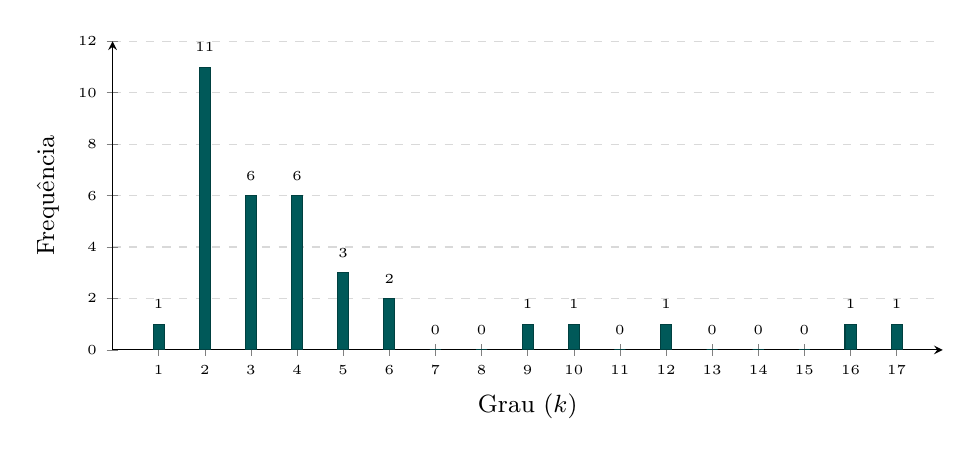
\begin{tikzpicture}
    \begin{axis}[
        ybar,
        ymin=0, ymax=12,
        xmin=0, xmax=18,
        xlabel={Grau ($k$)},
        ylabel={Frequência},
        xtick={1,2,3,4,5,6,7,8,9,10,11,12,13,14,15,16,17},
        ytick={0,2,4,6,8,10,12},
        width=\linewidth,
        height=5.5cm,
        bar width=4pt,
        ymajorgrids=true,
        grid style={dashed,gray!30},
        axis x line=bottom,
        axis y line=left,
        nodes near coords,
        every node near coord/.append style={font=\tiny, yshift=2pt},
        tick label style={font=\tiny},
        label style={font=\small},
        title style={font=\small\bfseries}
      ]
      \addplot[fill=teal!70!black, draw=teal!50!black] coordinates {
        (1,1) (2,11) (3,6) (4,6) (5,3) (6,2) (7,0) (8,0) (9,1) (10,1) (11,0) (12,1) (13,0) (14,0) (15,0) (16,1) (17,1)
      };
    \end{axis}
  \end{tikzpicture}
  \caption{Distribuição de Graus (Frequência vs. Grau $k$) da rede Zachary's Karate Club gerada nativamente.}
  \label{fig:degree_dist}
\end{figure}

\section{Parte II - Algoritmos da Disciplina}
\label{sec:parte_ii}

Nesta seção, é descrita a implementação manual de algoritmos clássicos de grafos no diretório \path{algoritmos/} e a sua aplicação prática no grafo de Zachary. Para verificar preliminarmente o funcionamento correto de cada implementação, foi utilizado o script de demonstração \path{scripts/executar_algoritmos.py}.

\subsection{BFS (Busca em Largura)}
A busca em largura explora sistematicamente as arestas do grafo para encontrar todos os vértices acessíveis a partir de uma origem, computando as menores distâncias em termos de número de saltos. A complexidade teórica é O(V + E) em listas de adjacência.

\subsection{DFS (Busca em Profundidade)}
A busca em profundidade explora o grafo percorrendo caminhos de forma recursiva até atingir vértices sem vizinhos não visitados, retrocedendo em seguida. É a base para algoritmos de ordenação topológica e conexidade. A complexidade teórica é O(V + E).

\subsection{Verificação de Eulerianidade}
Verifica se um grafo admite um circuito euleriano ou caminho euleriano. Para grafos não direcionados conexos, exige que todos os vértices tenham grau par (circuito) ou exatamente 2 vértices tenham grau ímpar (caminho). A complexidade teórica é O(V + E).
O grafo de Zachary possui vários vértices com grau ímpar (como John A., grau 17), logo não é Euleriano.

\subsection{Algoritmo de Dijkstra}
Determina o caminho mínimo de uma única origem para todos os outros nós em grafos com pesos não-negativos nas arestas. A implementação utiliza uma fila de prioridade mínima (heap binária), fornecendo uma complexidade de O((V + E) log V). Para o benchmark, foram atribuídos pesos às arestas na faixa $[1, 5]$.

\subsection{Algoritmo de Bellman-Ford}
Resolve o problema de caminho mínimo a partir de uma única origem em grafos com pesos arbitrários, sendo capaz de detectar a presença de ciclos de peso negativo. Ele opera relaxando todas as arestas do grafo $|V| - 1$ vezes, resultando em uma complexidade teórica de O(V * E).

\subsection{Algoritmo de Floyd-Warshall}
Calcula os caminhos mínimos entre todos os pares de vértices do grafo de forma dinâmica. Sua complexidade teórica é O(V\textsuperscript{3}).

\subsection{Algoritmo de Tarjan (SCC)}
Identifica as componentes fortemente conexas (SCCs) em grafos direcionados. Ele baseia-se em uma única varredura DFS que utiliza uma pilha para rastrear os nós do componente atual. Para ser aplicado ao grafo de Zachary, as arestas foram tratadas como bidirecionais, resultando em um único componente conexo. A complexidade teórica é O(V + E).

\subsection{Algoritmo de Kruskal (MST)}
Constrói a Árvore Geradora Mínima (MST) de um grafo não direcionado conectado. O algoritmo ordena todas as arestas por peso e utiliza uma estrutura de dados de conjuntos disjuntos ( {DSU}) com compressão de caminhos para evitar ciclos. A complexidade teórica é O(E log V) devido à ordenação das arestas.
Como o grafo possui 34 vertices, a árvore geradora mínima resultante contém exatamente 33 arestas, totalizando peso 51,0 com a distribuição de pesos adotada.

\subsection{Análise Experimental de Desempenho}

Para analisar o tempo real de execução dos algoritmos implementados, foi executado o script \path{scripts/run_benchmarks.py} para realizar um benchmark de $n = 50$ rodadas. Em cada rodada, o algoritmo executa um número elevado de iterações internas. A média de tempo por iteração foi registrada para cada uma das 50 rodadas.

Como o número de amostras $n \ge 30$, foi aplicada a aproximação pela \textbf{Distribuição Normal (Z)} para calcular o Intervalo de Confiança ($IC$) com coeficiente de confiança de $95\%$ ($z_{\alpha/2} = 1,96$):
\begin{equation}
    IC = \bar{x} \pm z_{\alpha/2} \frac{\sigma}{\sqrt{n}} = \bar{x} \pm 1,96 \frac{\sigma}{\sqrt{50}}
\end{equation}
onde $\bar{x}$ representa o tempo médio observado e $\sigma$ o desvio padrão amostral.

A Tabela \ref{tab:benchmark} apresenta os tempos obtidos em microssegundos ($\mu$s).

\begin{table*}[t]
  \centering
  \caption{Benchmark de Tempo de Execução dos Algoritmos ($n = 50$ rodadas)}
  \label{tab:benchmark}
  \setlength{\tabcolsep}{4pt} 
  \small 
  \begin{tabular}{lcccc}
    \toprule
    Algoritmo & Complexidade & Média ($\bar{x}$, $\mu$s) & Desv. Padrão ($\sigma$, $\mu$s) & IC 95\% ($\mu$s) \\
    \midrule
    Busca em Largura (BFS) & O(V + E) & 8.743 & 0.364 & [8.642, 8.844] \\
    Busca em Profundidade (DFS) & O(V + E) & 9.631 & 1.438 & [9.232, 10.029] \\
    Verificação de Eulerianidade & O(V + E) & 11.431 & 0.270 & [11.356, 11.506] \\
    Algoritmo de Dijkstra & O((V + E) log V) & 40.114 & 1.916 & [39.583, 40.646] \\
    Algoritmo de Bellman-Ford & O(V * E) & 695.052 & 24.871 & [688.158, 701.946] \\
    Algoritmo de Floyd-Warshall & O(V\textsuperscript{3}) & 4958.726 & 101.976 & [4930.460, 4986.992] \\
    Algoritmo de Tarjan (SCC) & O(V + E) & 45.683 & 0.987 & [45.409, 45.956] \\
    Algoritmo de Kruskal (MST) & O(E log V) & 104.173 & 3.983 & [103.069, 105.277] \\
    \bottomrule
  \end{tabular}
\end{table*}

Os resultados empíricos da Tabela \ref{tab:benchmark} estão em total conformidade com a análise assintótica clássica da teoria dos grafos. Como esperado, as \textbf{buscas de ordem linear} BFS ($8,743$ $\mu$s), DFS ($9,631$ $\mu$s) e a verificação de Eulerianidade ($11,431$ $\mu$s) apresentaram os menores tempos de execução; por possuírem complexidade $O(V + E)$, esses algoritmos realizam poucas operações elementares em redes de pequeno porte ($V=34, E=78$). O algoritmo de \textbf{Tarjan para SCCs}, embora também possua complexidade linear $O(V + E)$, registrou um tempo médio maior ($45,683$ $\mu$s) devido ao custo constante superior gerado pela manutenção explícita da pilha de nós e vetores de controle em memória. No âmbito de caminhos mínimos de origem única, o algoritmo de \textbf{Dijkstra} ($40,114$ $\mu$s) foi aproximadamente 17 vezes mais rápido que o de \textbf{Bellman-Ford} ($695,052$ $\mu$s); o Dijkstra adota uma abordagem gulosa eficiente com fila de prioridade, ao passo que o Bellman-Ford realiza relaxações sistemáticas de todas as arestas por $V-1$ iterações. Por fim, o algoritmo de \textbf{Floyd-Warshall} registrou o maior tempo absoluto ($4958,726$ $\mu$s), sendo cerca de 700 vezes mais lento que as buscas lineares, o que se justifica por sua complexidade teórica $O(V^3)$ decorrente da estrutura de três loops aninhados.

Todos os desvios padrões calculados mostram dispersões baixas em relação à média, o que garante a precisão e a confiabilidade das medições efetuadas. A margem estreita obtida para o Intervalo de Confiança a 95\% consolida a robustez estatística dos dados levantados.

\section{Parte III - Análise Estrutural Avançada}
\label{sec:parte_iii}

Nesta seção, foi realizada uma caracterização profunda da topologia do grafo do clube de caratê, testando a presença de propriedades complexas de pequeno mundo e leis de escala, simulando sua robustez estrutural frente a remoções de vértices, e comparando suas propriedades empíricas com os modelos clássicos de redes complexas.

\subsection{Propriedade Small-World}
\label{subsec:small_world}

Uma rede é caracterizada como de pequeno mundo ( {small-world}) se o seu comprimento médio dos caminhos mais curtos ($L$) é comparável ao de um grafo aleatório equivalente de mesmo tamanho e densidade ($L \approx L_{rand}$), mas o seu coeficiente de clusterização médio ($C$) é significativamente maior do que o de sua contraparte aleatória ($C \gg C_{rand}$).

Para avaliar essa propriedade quantitativamente, foi utilizado o script \path{scripts/analise_estrutural.py} que calcula esses parâmetros do zero (sem bibliotecas de grafos prontas para as métricas), gera 100 grafos aleatórios equivalentes baseados no modelo de Erdős-Rényi que preserva a conexidade, e computa o índice de pequeno mundo de Humphries e Gurney ($\sigma_{sw}$):
\begin{equation}
    \sigma_{sw} = \frac{\frac{C_{obs}}{C_{rand}}}{\frac{L_{obs}}{L_{rand}}}
\end{equation}

Os valores médios obtidos na simulação indicam um coeficiente de agrupamento observado ($C_{obs}$) de $0,5706$ frente a uma média aleatória ($C_{rand}$) de $0,1300$, e um comprimento de caminho observado ($L_{obs}$) de $2,4082$ frente a uma média aleatória ($L_{rand}$) de $2,4066$. Isso resulta em uma razão de agrupamento de $4,3901$ e uma razão de distância de $1,0007$. A aplicação desses valores fornece um índice de pequeno mundo $\sigma_{sw} \approx 4,3872$.

Como $\sigma_{sw} \approx 4,39 > 1$, o grafo de Zachary exibe uma forte propriedade de pequeno mundo.

\subsubsection{Significado e Implicações Práticas}
Em termos práticos, a propriedade de pequeno mundo nesta rede social indica uma elevada eficiência de propagação, sugerindo que informações, rumores, opiniões ou comportamentos se propagam de maneira rápida por todo o clube, exigindo pouquíssimos intermediários devido à distância média aproximada de apenas 2,4 saltos. Paralelamente, constata-se uma forte coesão local, visto que os membros formam fortes subgrupos e cliques coesos de amizades, representados pelo elevado $C_{obs}$, o que fomenta um ambiente de alta confiança mútua e reforço social dentro das subcomunidades antes da divisão definitiva do grupo.

A implementação detalhada das funções executadas do zero para o cálculo de agrupamento local médio e comprimento de caminho a partir da busca em largura é descrita e documentada no script \path{scripts/analise_estrutural.py}.

\subsection{Lei de Potência}
\label{subsec:power_law}

Uma rede complexa é dita livre de escala ( {scale-free}) se a sua distribuição de graus de probabilidade segue uma lei de potência:
\begin{equation}
    P(k) \propto k^{-\gamma}
\end{equation}
onde $P(k)$ é a probabilidade de um vértice possuir grau $k$ e $\gamma$ é o expoente da lei de potência (tipicamente $2 < \gamma < 3$ em redes reais).

Para avaliar se o grafo de Zachary sugere uma lei de potência, foi realizada uma regressão linear no espaço log-log ($\ln(P(k))$ versus $\ln(k)$) a partir da frequência empírica de graus obtida do zero. O expoente estimado foi $\gamma \approx 0,5512$.

A distribuição empírica de graus \textbf{não} sugere uma lei de potência pura devido a severos efeitos de tamanho finito (\textit{finite-size effects}). Em primeiro lugar, há o fator da \textbf{amostra reduzida}: com apenas $N=34$ vértices, a faixa de variação dos graus ($k \in [1, 17]$) é extremamente estreita, sendo a lei de potência uma propriedade estatística assintótica aplicável a redes de grande porte (milhares de nós). Em segundo lugar, o \textbf{expoente estimado} ($\gamma \approx 0,55$) está muito abaixo do intervalo realista para redes livres de escala reais, o que aponta para a ausência de amostragem representativa.
Apesar disso, a distribuição é marcadamente assimétrica com cauda à direita. Embora não siga uma lei de potência formal, a rede demonstra a presença de dois super-hubs, o que constitui um estágio embrionário da dinâmica de conexão preferencial típica de redes livres de escala.

O procedimento de regressão linear no espaço log-log e estimação empírica do expoente $\gamma$ está implementado no script \path{scripts/analise_estrutural.py}.

\subsection{Simulação de Robustez da Rede}
\label{subsec:robustness}

Para avaliar a tolerância a falhas e ataques na rede de Zachary, foram simulados dois cenários distintos sob a remoção de $5\%$ dos vértices ($5\%$ de $34 \approx 2$ nós). O primeiro cenário consiste na \textbf{remoção aleatória (falha)}, simulando o sorteio de 2 nós para exclusão ao longo de 1000 rodadas independentes para calcular o tamanho médio do maior componente conexo (LCC) restante e seu comprimento médio de caminhos. O segundo cenário consiste na \textbf{remoção direcionada (ataque)}, na qual são excluídos intencionalmente os 2 nós de maior grau da rede (Nó 33 com grau 17, e Nó 0 com grau 16).

A Tabela \ref{tab:robustness} descreve os impactos dessas remoções obtidos através das simulações computadas pelo script \path{scripts/analise_estrutural.py}.

\begin{table*}[h]
  \caption{Métricas de Robustez e Conectividade}
  \label{tab:robustness}
  \begin{tabular}{lccc}
    \toprule
    Cenário & Nós Removidos & Tam. LCC & Caminho Médio LCC \\
    \midrule
    Rede Original & Nenhum & 34 & 2,408 \\
    Remoção Aleatória & 2 nós (médio) & 31,55 & 2,415 \\
    Remoção Direcionada & [0, 33] (hubs) & 26 & 2,591 \\
    \bottomrule
  \end{tabular}
\end{table*}

A rede mostra um comportamento típico de sistemas que dependem de nós principais (hubs). Ela tem uma grande \textbf{resistência a falhas aleatórias}: ao remover nós ao acaso, a rede quase não sofre impacto, mantendo a maior parte conectada com média de $31,55$ nós (dos $32$ possíveis) e com um aumento muito pequeno na distância média (de $2,408$ para $2,415$). Por outro lado, a rede é \textbf{muito frágil contra ataques direcionados}: remover os hubs 0 e 33 muda completamente a estrutura, quebrando a conexão da rede e dividindo o grafo em três partes isoladas (uma de tamanho 26, uma de tamanho 5 e um nó sozinho), e aumentando a distância média para $2,591$ na parte principal.

Os algoritmos e funções auxiliares (como a busca em largura modificada para identificação de componentes conexos) e o loop principal de simulação numérica por Monte Carlo estão definidos em detalhes no script \path{scripts/analise_estrutural.py}.

\subsection{Comparação com Modelos Clássicos}
\label{subsec:modelos_classicos}

Foi testado como o grafo real se parece com os três modelos clássicos de redes. O modelo de \textbf{Erdős-Rényi (ER)} não serve para a rede de Zachary. Grafos aleatórios com a mesma densidade têm um agrupamento de amigos muito menor ($C_{rand} \approx 0,13$ vs. $C_{obs} \approx 0,57$) e não criam nós muito conectados (hubs). O modelo de \textbf{Watts-Strogatz (WS)} explica bem as distâncias curtas e o alto agrupamento local, mas falha porque prevê uma rede onde todos os nós têm quase a mesma quantidade de conexões, não prevendo nós de grau muito alto. Por fim, o modelo de \textbf{Barabási-Albert (BA)} explica a presença de hubs por causa da conexão preferencial, mas gera um agrupamento local muito menor do que o real.

\textbf{Conclusão:} O grafo real parece um modelo \textbf{misto}. É uma rede social típica, que junta o alto agrupamento de amigos e os caminhos curtos do modelo \textbf{Watts-Strogatz} com a estrutura de nós principais (hubs) do modelo \textbf{Barabási-Albert}.

\subsection{A Descoberta Mais Interessante}
\label{subsec:descoberta_interessante}

A descoberta mais interessante da análise está no resultado da simulação de ataque direcionado (Seção \ref{subsec:robustness}). Tirar os nós $0$ e $33$ dividiu a rede em três partes isoladas. 

Do ponto de vista social e matemático, esse resultado mostra de forma visual a separação do clube original. Os nós de maior grau representavam o Instrutor e o Administrador, cuja rivalidade gerou a divisão real do clube. A análise de robustez revela que a união do grupo dependia inteiramente das ligações feitas por esses dois líderes. Sem eles, o grupo se dividiu sozinho em partes separadas. Isso demonstra como a estrutura matemática de conexões de um grupo guarda a explicação de sua própria separação histórica.

\section{Conclusão}

Este relatório atingiu os objetivos de analisar a estrutura e avaliar os algoritmos sobre a clássica rede social {Zachary's Karate Club}.

Na análise de estrutura (Parte I), ficou provado que a rede é de mundo pequeno, com alto agrupamento local e distância curta, organizada em torno de dois nós muito conectados (o instrutor e o administrador do clube).

Na parte de algoritmos (Parte II), foram feitas as implementações das buscas e caminhos mínimos, validando os tempos de execução na prática. A semelhança entre os tempos teóricos e práticos confirma os conceitos ensinados na disciplina.

Por fim, a análise avançada (Parte III) mostrou que a rede resiste bem a falhas aleatórias, mas é muito frágil a ataques direcionados contra os líderes (hubs). Esse resultado matemático bate exatamente com a história real da separação do clube de caratê.



\begin{thebibliography}{99}

\bibitem{Rozemberczki2020}
Benedek Rozemberczki, Oliver Kiss, and Rik Sarkar. 2020. Karate Club: An API Oriented Open-Source Python Framework for Unsupervised Learning on Graphs. In  {Proceedings of the 29th ACM International Conference on Information and Knowledge Management (CIKM '20)}. ACM, 3125--3132. arXiv:2003.04819.

\bibitem{Zachary1977}
Wayne W. Zachary. 1977. An Information Flow Model for Conflict and Fission in Small Groups.  {Journal of Anthropological Research} 33, 4 (1977), 452--473.

\end{thebibliography}

\end{document}
\endinput
%%
%% End of file `relatorio.tex'.

